\documentclass[a4paper, 12pt]{article}

% Includes 
\usepackage[utf8]{inputenc} % UTF-8 encode 
\usepackage[english, russian]{babel}
\usepackage{geometry} % adjust page layout 
\usepackage{graphicx} 
\usepackage{hyperref} 
\usepackage{amsmath} % math formulas 
\usepackage{setspace} % for set line spacing 
\usepackage{indentfirst} % indent on a first line after the paragraph 
\usepackage{pgfplots} % for plots 
\usepackage{listings} % for code listings 
\usepackage{xcolor} % colors (used for listings)
\usepackage{sourcecodepro} % for another monospaced font 
\usepackage{float}

\usepackage{amssymb}

% debug
% \usepackage{showframe} % frame borders for demonstration 


%%% Custom commands
% commands for unnumbered sections
\newcommand{\usection}[1]{\section*{#1} \addcontentsline{toc}{section}{\protect\numberline{}#1}}
\newcommand{\usubsection}[1]{\subsection*{#1} \addcontentsline{toc}{subsection}{\protect\numberline{}#1}}
\newcommand{\usubsubsection}[1]{\subsubsection*{#1} \addcontentsline{toc}{subsubsection}{\protect\numberline{}#1}}

% Redefinition of section and subsection numbering style
\def\thesection{\arabic{section}.}
\def\thesubsection{\arabic{section}.\arabic{subsection}.}
\def\thesubsubsection{\arabic{section}.\arabic{subsection}.\arabic{subsubsection}.}

%%% ------------------------ %%% 

%%% Settings for links 
\hypersetup{
	colorlinks,
	citecolor=black,
	filecolor=black,
	linkcolor=black,
	urlcolor=blue
}


% Layout
\geometry{
	left=17mm,
	top=17mm,
	right=17mm,
	bottom=20mm,
	marginparsep=0mm,
	marginparwidth=0mm,
	headheight=8mm,
	headsep=5mm, 
}

\linespread{1.5} % line spacing
\setlength{\parskip}{\baselineskip}  % Add space between paragraphs


%%% Overfull hbox settings
\tolerance 10000 % default 1000, max 10000
\hbadness 10000 % default 1000, max 10000
\emergencystretch 0pt  % default 0pt, how much the lines can stretch for the sake of good line breaks
\hfuzz 0.4pt % ignore overfull box less than 
\widowpenalty=0 % default 1000, max 10000
\vfuzz \hfuzz % don't care about underfull vbox if overfull is acceptable
% \raggedbottom % if the page is not filled, align the content to the bottom


%%% Redefinition of table of contents command to get centered heading
\makeatletter
\renewcommand\tableofcontents{ 
	\begin{singlespace}
		\null\hfill\textbf{\Large\contentsname}\hfill\null\par
		\@mkboth{\MakeUppercase\contentsname}{\MakeUppercase\contentsname}%
		\@starttoc{toc}
	\end{singlespace}
}
\makeatother


%%% Listings settings
\definecolor{codegreen}{rgb}{0, 0.6, 0}
\definecolor{codegray}{rgb}{0.5, 0.5, 0.5}
\definecolor{codepurple}{rgb}{0.58, 0, 0.82}
\definecolor{backcolour_gray}{rgb}{0.98, 0.98, 0.98}

\lstdefinestyle{python_white}{
	language=Python,
	backgroundcolor=\color{backcolour_gray},   
	commentstyle=\color{codegreen},
	keywordstyle=\color{blue},
	numberstyle=\tiny\color{codegray},
	stringstyle=\color{codepurple},
	basicstyle=\ttfamily\small\singlespacing,
	breakatwhitespace=true,         
	breaklines=true,                 
	captionpos=b, % t/b                  
	keepspaces=true,                 
	numbers=none, % none/left/rigth                    
	numbersep=5pt,                  
	showspaces=false,                
	showstringspaces=false,
	showtabs=false,                  
	tabsize=2,
	frame=single, % none/leftline/topline/bottomline/lines/single/shadowbox
	rulecolor=\color{gray}, % frame color 
	belowskip=-1\baselineskip % space after the listing
}


\lstset{style=python_white}


%%% For plots 
\pgfplotsset{width=10cm,compat=1.9}


%%% ------------------------ %%% 

% For title page
\def\name{Отчет по лабораторной работе №2} 
\def\subname{Модальные регуляторы и наблюдатели}
\def\variant{19}
\def\nameu{Новичков Дмитрий, R3335}
\def\teacher{Пашенко А. В.}

\begin{document}
	
	% Title page 
\begin{titlepage}

  \thispagestyle{empty}
  
  \title{


  
\includegraphics[width=4cm]{media/ITMO_logo.png} 

  \begin{center}
  \large\textsc{\textbf{Национальный исследовательский университет ИТМО}}
  \vspace{2em}
  \end{center}


  \begin{center}
    \large\textsc{\textbf{\name}}

    ``\subname'' 

    \large\textsc{\textbf{по дисциплине: Теория автоматического управления}}
    
    Вариант \variant
  \end{center}
  
  
  \vspace{3em}
  
  \begin{flushright}
  \normalsize{ 
  Выполнил: \\ \textbf{\nameu} \\
  Преподаватель: \\ \textbf{\teacher} 
  }
  \end{flushright}	
  
  \vfill
  
  \begin{center}
  \small{Санкт-Петербург, \the\year}
  \end{center}
  }
  
  
  \author{}
  \date{}
  \maketitle
  \thispagestyle{empty}
  \end{titlepage} % Title page
	
	\tableofcontents % Table of contents
	\pagebreak

	\section{Модальный регулятор}

Рассмотрим систему $\dot{x} = Ax + Bu$, где 
\begin{equation}
    \begin{gathered}
        A = \begin{bmatrix}
            4 & 6 & 4 \\
            -4 & -6 & -6 \\
            4 & 4 & 4
        \end{bmatrix}, \quad
        B = \begin{bmatrix}
            4 \\
            -1 \\
            1
        \end{bmatrix}, \quad
        \begin{cases}
            \sigma_1 &= \{-1, -1, -1\} \\
            \sigma_2 &= \{-2, -2, -2\} \\
            \sigma_3 &= \{-1, -10, -100\} \\
            \sigma_4 &= \{-2, -20, -200\} \\
            \sigma_5 &= \{-1, -1 - 3i, -1 + 3i\} \\
            \sigma_6 &= \{-2, -2 - 6i, -2 + 6i\}
        \end{cases}
    \end{gathered}
\end{equation}

\subsection{Управляемость системы}

\subsubsection{Управляемость собственных значений}
Найдем спектр матрицы $A$:
\begin{equation}
    \sigma(A) = \{-2, 2-2j, 2+2j\}
\end{equation}

Для каждого собственного значения найдем матрицу Хаутуса $H_i = \begin{bmatrix} A - \lambda_i I & B \end{bmatrix}$ и определим ее ранг:
\begin{enumerate}
    \item $\lambda_1 = -2$: $H_1 = \begin{bmatrix}
        6 & 6 & 4 & 4\\
        -4 & -4 & -6 & -1 \\
        4 & 4 & 6 & 1
    \end{bmatrix}$, $\text{rank}(H_1) = 2$, собственное значение неуправляемо.
    \item $\lambda_2 = 2-2j$: $H_2 = \begin{bmatrix}
        2+2j & 6 & 4 & 4\\
        -4 & -4+2j & -6 & -1 \\
        4 & 4 & 6+2j & 1
    \end{bmatrix}$, $\text{rank}(H_2) = 3$, собственное значение управляемо.
    \item $\lambda_3 = 2+2j$: $H_3 = \begin{bmatrix}
        2+2j & 6 & 4 & 4\\
        -4 & -4+2j & -6 & -1 \\
        4 & 4 & 6+2j & 1
    \end{bmatrix}$, $\text{rank}(H_3) = 3$, собственное значение управляемо.
\end{enumerate}

Собственное число $\lambda_1$ является \textbf{неуправляемым}. Следовательно, согласно критерию Хаутуса, система \textbf{не является полностью управляемой}.  
Однако система будет \textbf{стабилизируемой}, так как все \textbf{неустойчивые собственные числа} (если таковые имеются) оказываются \textbf{управляемыми}.

\subsection{Достижимые спектры}
Не все спектры могут быть использованы в качестве достижимых для матрицы замкнутой системы $(A + BK)$, так как система \textbf{не является полностью управляемой}. Это ограничение связано с неуправляемым собственным числом $\lambda_3 = -2$, которое \textbf{нельзя изменить с помощью регулятора}. Следовательно, $\lambda_3$ обязательно останется одним из собственных чисел матрицы $(A + BK)$ после замыкания системы. После отбора доступных спектров остаются следующие, которые уже являются достижимыми:

\[
\sigma_2 = \{-2, -2, -2\}, \quad
\sigma_4 = \{-2, -20, -200\}, \quad
\sigma_6 = \{-2, -2 - 6i, -2 + 6i\}.
\]

\subsubsection{Первый спектр}
Задан желаемый спектр замкнутой системы:
\[
\sigma_1 = \{-2, -2, -2\}.
\]

Для нахождения матрицы регулятора $K$, которая обеспечивает данный спектр, воспользуемся следующей системой уравнений:
\[
\begin{cases}
AP - PG = BY, \\
K = -Y P^{-1},
\end{cases}
\]
где:
\begin{itemize}
    \item $P$ — матрица преобразования,
    \item $G$ — матрица с желаемым спектром,
    \item $Y$ — вспомогательная матрица.
\end{itemize}

Перед синтезом регулятора убедимся, что выполняются следующие условия:
\begin{enumerate}
    \item Спектры матриц $A$ и $G$ не пересекаются: $\sigma(A) \cap \sigma(G) = \emptyset$.
    \item Пара $(A, B)$ является управляемой (или хотя бы стабилизируемой).
    \item Пара $(Y, G)$ является наблюдаемой.
\end{enumerate}

Матрицы $G$ и $Y$ выбираются следующим образом:
\begin{itemize}
    \item $G \in \mathbb{R}^{n \times n}$ — матрица с желаемым спектром $\sigma(G)$.
    \item $Y \in \mathbb{R}^{m \times n}$ — матрица, обеспечивающая наблюдаемость пары $(Y, G)$.
\end{itemize}

Затем решаем уравнение Сильвестра $AP - PG = BY$ для нахождения $P$ и вычисляем регулятор $K = -Y P^{-1}$.

В нашем случае пара $(A, B)$ является \textbf{стабилизируемой}, но не полностью управляемой. Это означает, что решение может быть не единственным или вырожденным. Однако, выбрав $G$ и $Y$ следующим образом:
\[
G = \begin{bmatrix}
-2 & 1 & 0 \\
0 & -2 & 1 \\
0 & 0 & -2
\end{bmatrix}, \quad
Y = \begin{bmatrix}
1 & 0 & 1
\end{bmatrix},
\]
мы обеспечиваем выполнение всех необходимых условий.

После вычислений получаем коэффициенты регулятора:
\[
K = \begin{bmatrix}
-1.94 & -1.94 & -1.94
\end{bmatrix}.
\]
\newpage
Собственные числа матрицы замкнутой системы $(A + BK)$ :
\[
\lambda_{1,2,3} \approx -2,
\]
что соответствует заданному спектру $\sigma_1$. Это подтверждает корректность синтеза регулятора.

\begin{figure}[H]
    \centering
    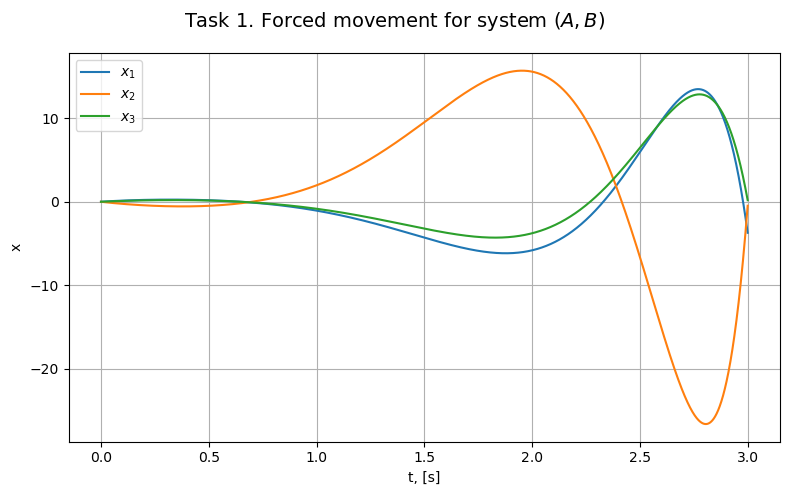
\includegraphics[width=0.8\textwidth]{../../plots/task_1_1.png}
    \caption{Состояние системы}
    \label{fig:task_1_state_system_1}
\end{figure}

\begin{figure}[H]
    \centering
    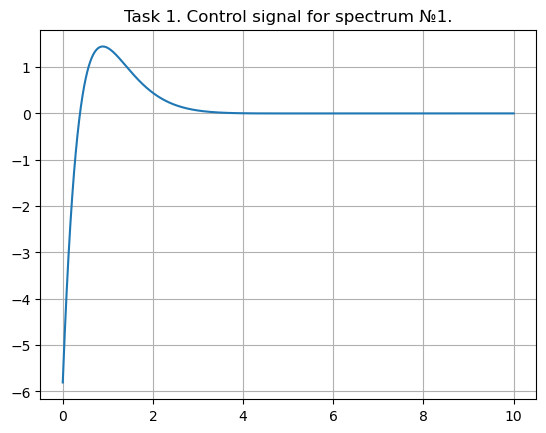
\includegraphics[width=0.8\textwidth]{../../plots/task_1_2.png}
    \caption{Сигнал управления}
    \label{fig:task_1_control_signal_1}
\end{figure}

\subsubsection{Второй спектр}

Рассмотрим второй желаемый спектр замкнутой системы:
\[
\sigma_2 = \{-2, -20, -200\}.
\]

Для нахождения матрицы регулятора $K$ воспользуемся следующей системой уравнений:
\[
\begin{cases}
AP - PG = BY, \\
K = -Y P^{-1},
\end{cases}
\]
где:
\begin{itemize}
    \item $P$ — матрица преобразования,
    \item $G$ — матрица с желаемым спектром,
    \item $Y$ — вспомогательная матрица.
\end{itemize}

Для решения системы выберем матрицы $G$ и $Y$ следующим образом:
\[
G = \begin{bmatrix}
-2 & 0 & 0 \\
0 & -20 & 0 \\
0 & 0 & -200
\end{bmatrix}, \quad
Y = \begin{bmatrix}
0 & 1 & 1
\end{bmatrix}.
\]

После выполнения вычислений получаем коэффициенты регулятора:
\[
K = \begin{bmatrix}
26.08 & 164.16 & -164.16
\end{bmatrix}.
\]

Собственные числа матрицы замкнутой системы $(A + BK)$:
\[
\lambda_1 = -2, \quad \lambda_2 = -20, \quad \lambda_3 = -200.
\]

Эти значения соответствуют заданному спектру $\sigma_2$, что подтверждает корректность синтеза регулятора.

\begin{figure}[H]
    \centering
    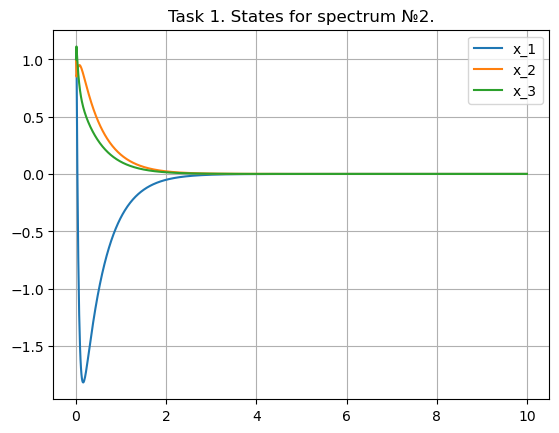
\includegraphics[width=0.8\textwidth]{../../plots/task_1_3.png}
    \caption{Состояние системы}
    \label{fig:task_1_state_system_2}
\end{figure}

\begin{figure}[H]
    \centering
    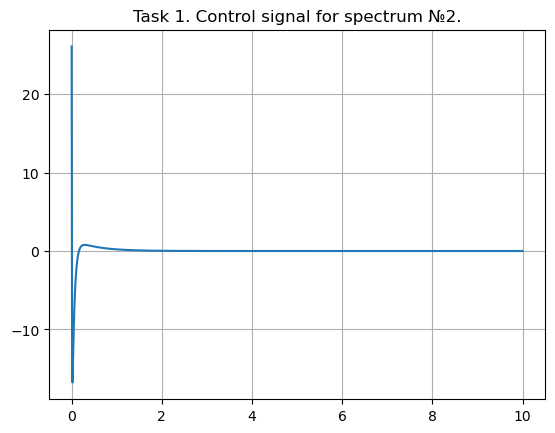
\includegraphics[width=0.8\textwidth]{../../plots/task_1_4.png}
    \caption{Сигнал управления}
    \label{fig:task_1_control_signal_2}
\end{figure}


\subsubsection{Третий спектр}

Рассмотрим третий желаемый спектр замкнутой системы:
\[
\sigma_2 = \{-2, -2-6j, -2+6j\}.
\]

Для нахождения матрицы регулятора $K$ воспользуемся следующей системой уравнений:
\[
\begin{cases}
AP - PG = BY, \\
K = -Y P^{-1},
\end{cases}
\]
где:
\begin{itemize}
    \item $P$ — матрица преобразования,
    \item $G$ — матрица с желаемым спектром,
    \item $Y$ — вспомогательная матрица.
\end{itemize}

Для решения системы выберем матрицы $G$ и $Y$ следующим образом:
\[
G = \begin{bmatrix}
-2 & 0 & 0 \\
0 & -2 & 6 \\
0 & -6 & -2
\end{bmatrix}, \quad
Y = \begin{bmatrix}
0 & 1 & 1
\end{bmatrix}.
\]

После выполнения вычислений получаем коэффициенты регулятора:
\[
K = \begin{bmatrix}
-1.28 & 1.44 & -1.44
\end{bmatrix}.
\]

Собственные числа матрицы замкнутой системы $(A + BK)$:
\[
\lambda_1 = -2, \quad \lambda_2 = -2-6j, \quad \lambda_3 = -2+6j.
\]

Эти значения соответствуют заданному спектру $\sigma_3$, что подтверждает корректность синтеза регулятора.

\begin{figure}[H]
    \centering
    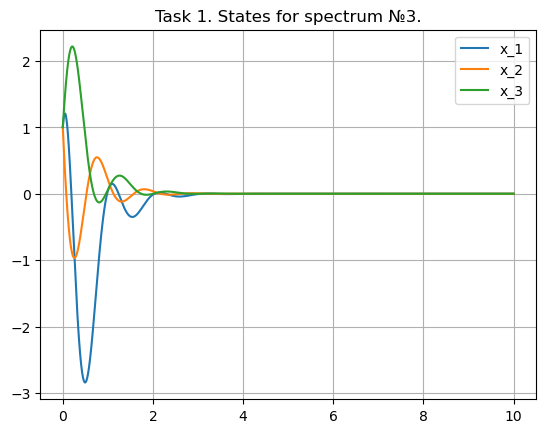
\includegraphics[width=0.8\textwidth]{../../plots/task_1_5.png}
    \caption{Состояние системы}
    \label{fig:task_1_state_system_3}
\end{figure}

\begin{figure}[H]
    \centering
    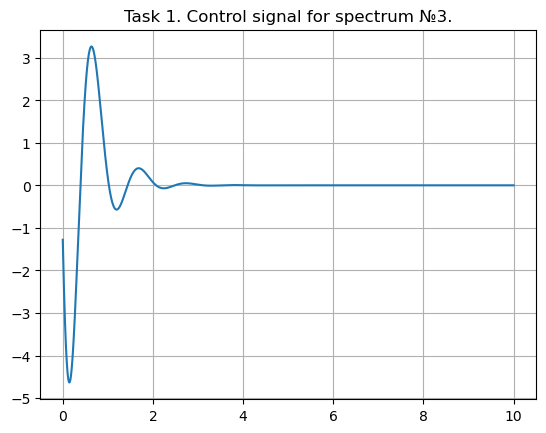
\includegraphics[width=0.8\textwidth]{../../plots/task_1_6.png}
    \caption{Сигнал управления}
    \label{fig:task_1_control_signal_3}
\end{figure}


\subsection{Сравнение выбора спектра для синтеза регулятора}

\subsubsection{Первый спектр}
Мы выбрали относительно небольшие устойчивые моды. В результате регулятор корректировал систему плавно, с минимальным перерегулированием. Это обеспечило стабильное и предсказуемое поведение системы.

\subsubsection{Второй спектр}
Для ускорения процесса управления мы значительно увеличили моды. Это привело к агрессивному управлению, которое быстро привело систему в нулевую позицию. Однако в реальных условиях такое управление может быть неприменимо из-за физических ограничений

\subsubsection{Третий спектр}
В спектр были включены комплексно-сопряжённые моды. Это привело к сходимости системы с небольшими колебаниями, но в целом плавно и с умеренным перерегулированием. Вещественная часть этих мод не слишком велика, что обеспечивает баланс между скоростью и стабильностью.


\subsection{Вывод}
Проведённое исследование системы показало, что даже \textbf{стабилизируемая система} (которая не обязательно является полностью управляемой) позволяет реализовать управление с различными характеристиками сходимости. Мы успешно синтезировали \textbf{модальный регулятор}, используя уравнение Сильвестра. Совпадение желаемых спектров со спектром матрицы замкнутой системы $(A + BK)$ подтверждает корректность выполненного синтеза.
	\section{Управляемое подпространство}

Рассмотрим систему $\dot{x} = Ax + Bu$, где 
\begin{equation}
    \begin{array}{ccc}
        A = \begin{bmatrix}
            7 & -7 & 8 \\
            6 & -5 & 6 \\
            -6 & 4 & -7
        \end{bmatrix}, &
        B = \begin{bmatrix}
            -3 \\
            -1 \\
            1
        \end{bmatrix}, &
        x_1' = \begin{bmatrix}
            -8 & 3 & 0
        \end{bmatrix},
        x_1'' = \begin{bmatrix}
            -4 & 0 & 0
        \end{bmatrix},
    \end{array}
\end{equation}

\subsection{Управляемость системы}
\subsubsection{Матрица управляемости}
Найдем матрицу управляемости $U = [B, AB, A^2B]$:
\begin{equation}
    U = \begin{bmatrix} 
        \begin{array}{c|c|c}
            \begin{bmatrix}
                -3 \\
                -1 \\
                1
            \end{bmatrix} & 
            \begin{bmatrix}
                7 & -7 & 8 \\
                6 & -5 & 6 \\
                -6 & 4 & -7
            \end{bmatrix} \times 
            \begin{bmatrix}
                -3 \\
                -1 \\
                1
            \end{bmatrix} &
            \begin{bmatrix}
                7 & -7 & 8 \\
                6 & -5 & 6 \\
                -6 & 4 & -7
            \end{bmatrix}^2 \times
            \begin{bmatrix}
                -3 \\
                -1 \\
                1
            \end{bmatrix}
        \end{array}   
    \end{bmatrix}
\end{equation}
\begin{equation}
    U = \begin{bmatrix}
    3 & 36 & -183 \\ 
    -1 & 29 & -103 \\ 
    1 & -29 & 103 \\ 
    \end{bmatrix}
\end{equation}
Определим ранг матрицы управляемости:
\begin{equation}
    \text{rank}(U) = 2
\end{equation}
Так как ранг матрицы управляемости меньше размерности матрицы $A$, система не является полностью управляемой. 

\subsubsection{Управляемость собственных значений}
Определим управляемость собственных значений матрицы $A$. Для каждого собственного значения найдем матрицу Хаутуса $H_i = \begin{bmatrix} A - \lambda_i I & B \end{bmatrix}$ и определим ее ранг:
\begin{enumerate}
    \item $\lambda_1 = -1$: $H_1 = \begin{bmatrix}
        8 & -2 & 8 & -3\\
        4 & -4 & 4 & -1 \\
        -4 & 0 & -6 & 1
    \end{bmatrix}$, $\text{rank}(H_1) = 2$, собственное значение не управляемо.
    \item $\lambda_2 = -2-3j$: $H_2 = \begin{bmatrix}
        9+2j & -2 & 8 & -3\\
        4 & -3+2j & 4 & -1 \\
        -4 & 0 & -5+2j & 1
    \end{bmatrix}$, $\text{rank}(H_2) = 3$, собственное значение управляемо.
    \item $\lambda_3 = -2+3j$: $H_3 = \begin{bmatrix}
        9-2j & -2 & 8 & -3\\
        4 & -3-2j & 4 & -1 \\
        -4 & 0 & -5-2j & 1
    \end{bmatrix}$, $\text{rank}(H_3) = 3$, собственное значение управляемо.
\end{enumerate}

\subsubsection{Диагональная форма системы}
\begin{equation}
    \dot{\hat{x}} = \begin{bmatrix}
        -1 & 0 & 0 \\
        0 & -2-3j & 0 \\
        0 & 0 & -2+3j
    \end{bmatrix} \hat{x} + 
    \begin{bmatrix}
        0 \\
        \frac{1 - 9j}{2} \\ 
        \frac{1 + 9j}{2}
    \end{bmatrix} u
\end{equation}
Первое число в векторе $P^{-1}B$ равно нулю, значит, что первое состояние системы не является управляемым. 
Результаты совпали с результатами, полученными при анализе управляемости собственных значений через матрицу Хаутуса.

\subsection{Грамиан управляемости}
Найдем грамиан управляемости $P(t_1)$:
\begin{equation}
    P(t_1) = \int_{0}^{t_1} e^{At}BB^Te^{A^Tt}dt
\end{equation}
Вычислим грамиан управляемости для $t_1 = 3$ с помощью функции \texttt{gram}: 
\begin{equation}
    P(3) = \begin{bmatrix}
        23.29 & 11.16 & -11.16 \\ 
        11.16 & 6.14 & -6.14 \\ 
        -11.16 & -6.14 & 6.14 \\ 
    \end{bmatrix}
\end{equation}

Найдем собственные числа Грамиана управляемости:
\begin{equation}
   \sigma(P(3)) = \{0, 1.07, 34.49 \}
\end{equation}
Первое собственное число равно нулю, что говорит о том, что Грамиан является вырожденным и система не является полностью
управляемой. Таким образом, для дальнейшего нахождения управления необходимо использовать псведообратную матрицу. 

\subsection{Управляемое подпространство}
Выясним, принадлежат ли точки $x_1'$ и $x_1''$ управляемому подпространству:
\begin{equation}
    \begin{array}{cc}
        x_1' = \begin{bmatrix}
            -8 \\
            3 \\
            0
        \end{bmatrix}, &
        x_1'' = \begin{bmatrix}
            -4 \\
            0 \\
            0
        \end{bmatrix}
    \end{array}
\end{equation}

Для этого можно записать расширенную матрицу управляемости $U'$ и найти ранг этой матрицы:
\begin{equation}
    U' = \begin{bmatrix}
        3 & 36 & -183 & -8 \\ 
        -1 & 29 & -103 & 3 \\ 
        1 & -29 & 103 & 0 \\ 
    \end{bmatrix}
\end{equation}
\begin{equation}
    \text{rank}(U') = 3
\end{equation}

\begin{equation}
   U'' = \begin{bmatrix}
        3 & 36 & -183 & -4 \\ 
        -1 & 29 & -103 & 0 \\ 
        1 & -29 & 103 & 0 \\
    \end{bmatrix}
\end{equation}
\begin{equation}
    \text{rank}(U'') = 2
\end{equation}

Таким образом, можно сделать вывод, что точка $x_1''$ принадлежит управляемому подпространству, а точка $x_1'$ не принадлежит. В дальнейшем будем обозначать $x_1''$ как $x_1$.

\subsection{Управление системой}
Найдем управление $u(t)$, которое будет переводить систему из состояния $x(0) = 0$ в состояние $x_1 = x(t_1) = \begin{bmatrix} -8 & 3 & 0 \end{bmatrix}^T$. 
\begin{equation}
    u(t) = B^Te^{A^T(t_1 - t)}P(t_1)^{-1}x_1
\end{equation}

\begin{figure}[H]
    \centering
    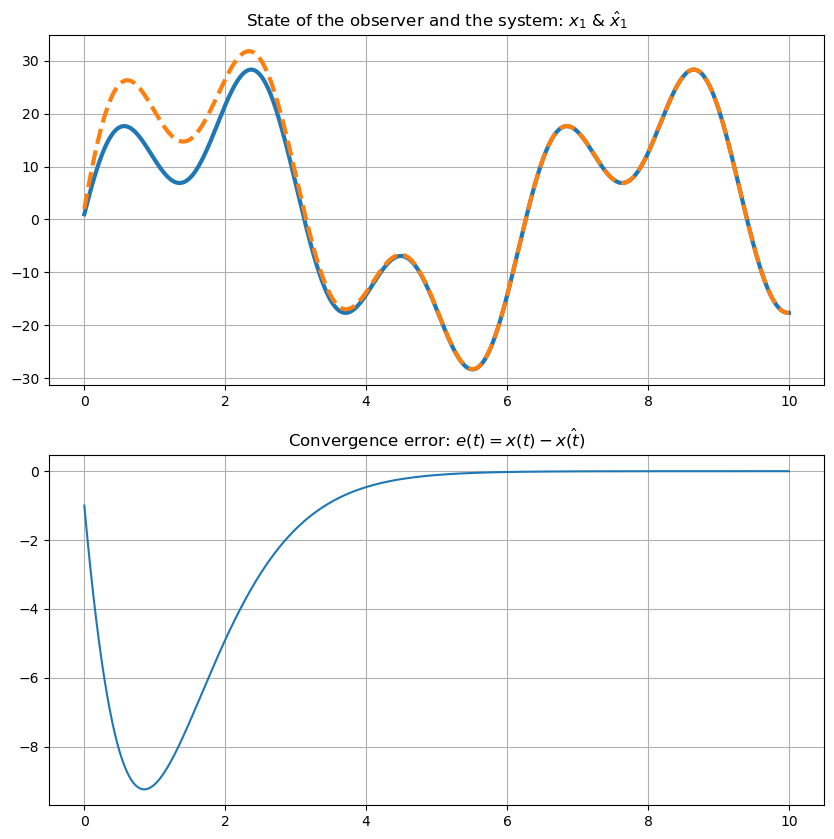
\includegraphics[width=0.9\textwidth]{../../plots/task_2_1.png}
    \caption{Управление системой}
    \label{fig:task2_control_signal}
\end{figure}

\begin{figure}[H]
    \centering
    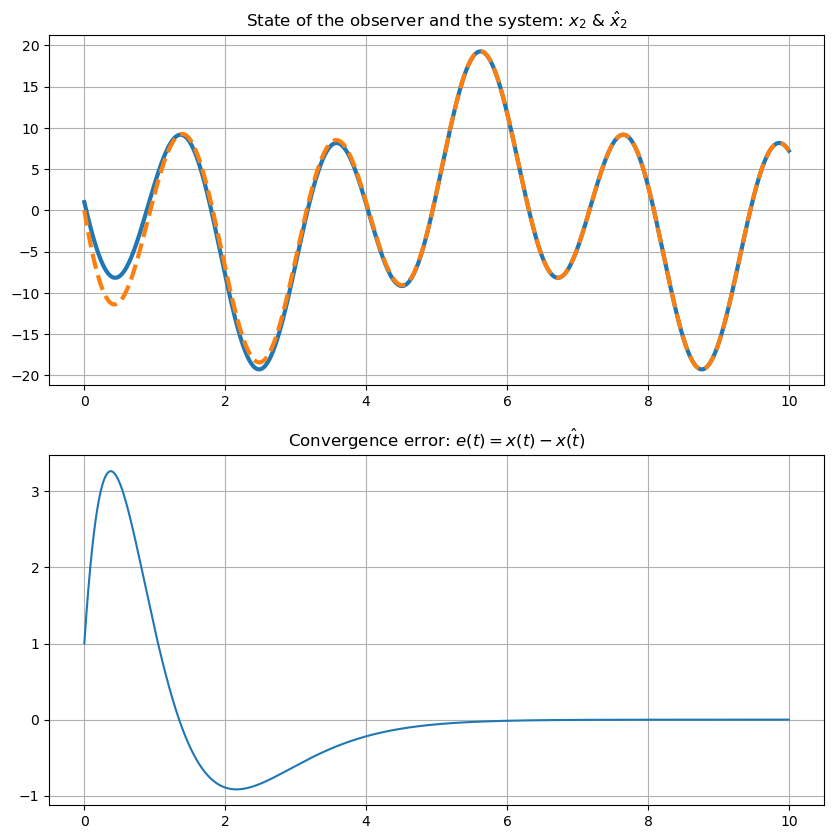
\includegraphics[width=0.9\textwidth]{../../plots/task_2_2.png}
    \caption{Состояние системы}
    \label{fig:task2_state}
\end{figure}

\subsection{Вывод}
В ходе исследования системы, представленной в данной задаче, было установлено, 
что она не является полностью управляемой. 
Это подтверждено с использованием критерия Калмана, 
а также анализом управляемости собственных значений и диагональной формы системы. 
В частности, выяснилось, что собственное число $\lambda_1 = -1$ не является 
управляемым. Дополнительно был вычислен грамиан управляемости, 
и проверка его собственных чисел показала, что одно из них равно нулю, 
что также свидетельствует о неполной управляемости системы.

Были рассмотрены две точки $x_1'$ и $x_2''$, и проведена проверка их принадлежности 
управляемому подпространству. Оказалось, что точка $x_1''$ принадлежат управляемому подпространству
в то время как точка $x_1'$ ему не принадлежит. 
	\section{Модальное управление по выходу.}

Исследуемая система описывается уравнениями:
\[
\begin{cases}
    \dot{x} = Ax + Bu, \\
    y = Cx + D,
\end{cases}
\]
где:
\begin{itemize}
    \item $x$ — вектор состояния системы,
    \item $u$ — входной сигнал (управление),
    \item $y$ — выходной сигнал.
\end{itemize}

Матрицы системы заданы следующим образом:

\[
A = \begin{bmatrix}
    5 & -7 & -5 & 1 \\
    -7 & 5 & -1 & 5 \\
    -5 & -1 & 5 & 7 \\
    1 & 5 & 7 & 5
\end{bmatrix}, \quad
B = \begin{bmatrix}
    5 \\
    7 \\
    1 \\
    9
\end{bmatrix}, \quad
C = \begin{bmatrix}
    0 & 0 & 2 & 2 \\
    1 & 1 & -1 & -1 \\
\end{bmatrix}
D = \begin{bmatrix}
    4 \\
    2 \\
\end{bmatrix}
\]


\subsection{Исследование наблюдаемости системы}

Для начала найдём матрицу наблюдаемости системы:
\[
V = \begin{bmatrix}
    C \\
    CA \\
    CA^2
\end{bmatrix} =
\begin{bmatrix}
    1 & 0 & 2 \\
    4 & -3 & 2 \\
    -11 & -6 & 16
\end{bmatrix}.
\]
Ранг матрицы наблюдаемости $V$ равен 3. Согласно критерию Калмана, система является \textbf{полностью наблюдаемой}, так как ранг матрицы наблюдаемости равен порядку системы.

Найдём собственные числа матрицы $A$:
\[
\sigma(A) = \{-8, 4, 8, 16\}.
\]

\subsection{Синтез наблюдателя и регулятора}

Выберем следующие спектры для наблюдателя и регулятора, которые обеспечат асимптотическую устойчивость замкнутой системы:
\[
\sigma(G_{\text{ctrl}}) = \{-1, -3, -3, -3\}, \quad
\sigma(G_{\text{obsv}}) = \{-1, -3, -3, -3\}.
\]

Используя метод синтеза регулятора и наблюдателя через уравнения Сильвестра, получим следующие матрицы $K$ и $L$:

\[
G_{\text{ctrl}} = \begin{bmatrix}
    -1 & 0 & 0 & 0 \\
    0 & -3 & 1 & 0 \\
    0 & 0 & -3 & 1 \\
    0 & 0 & 0 & -3
\end{bmatrix}, \quad
Y = \begin{bmatrix}
    1 \\
    1 \\
    1 \\
    1
\end{bmatrix}^T, \quad
K = \begin{bmatrix}
    8.51 \\
    -8.91 \\
    -0.87 \\
    -1.36
\end{bmatrix}^T.
\]

\[
G_{\text{obsv}} = \begin{bmatrix}
    -1 & 0 & 0 & 0 \\
    0 & -3 & 1 & 0 \\
    0 & 0 & -3 & 1 \\
    0 & 0 & 0 & -3
\end{bmatrix}, \quad
Y = \begin{bmatrix}
    1 & 1 \\
    1 & 1 \\
    0 & 0 \\
    1 & 1
\end{bmatrix}, \quad
L = \begin{bmatrix}
    35.60 & 35.60 \\
    -38.39 & -38.39 \\
    -12.02 & -12.02 \\
    -15.18 & -15.18
\end{bmatrix}.
\]

\subsection{Проверка корректности синтеза}

Вычислим собственные числа матриц регулятора $(A + BK)$ и наблюдателя $(A + LC)$:

\subsubsection{Собственные числа наблюдателя}
\[
    \sigma(A + LC) \approx \{-1, -3.0005, -2.9997 \pm 0.0004i\}.
\]

\subsubsection{Собственные числа регулятора}
\[
    \sigma(A + BK) \approx \{-1, -3.9996, -4.0002 \pm 0.0004i\}.
\]

Спектры практически совпадают с заданными, за исключением незначительных погрешностей. Это подтверждает корректность синтеза как регулятора, так и наблюдателя.


\subsection{Моделирование системы}

Проведём моделирование системы с начальными условиями:
\begin{itemize}
    \item Вектор состояния системы: $x(0) = \begin{bmatrix} 1 & 1 & 1 & 1 \end{bmatrix}^T$.
    \item Вектор состояния наблюдателя: $\hat{x}(0) = \begin{bmatrix} 0 & 0 & 0 & 0 \end{bmatrix}^T$.
\end{itemize}

\begin{figure}[H]
    \centering
    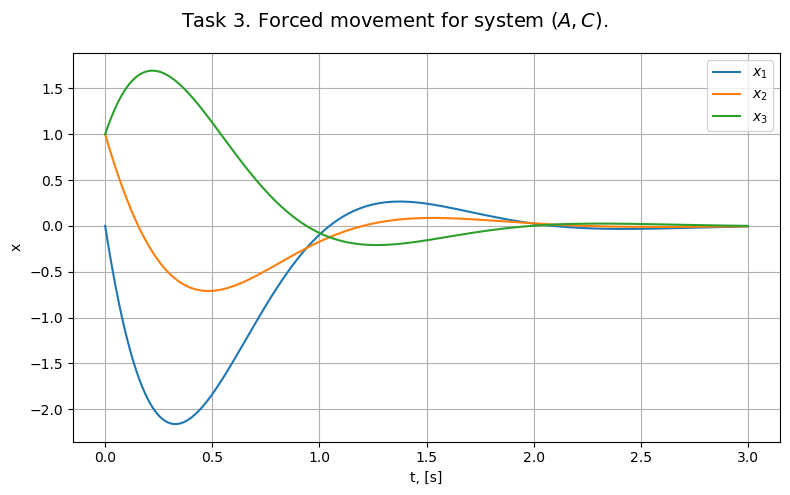
\includegraphics[width=0.7\textwidth]{../../plots/task_3_1.png}
    \caption{Состояние системы}
    \label{fig:task_3_state_system}
\end{figure}

\begin{figure}[H]
    \centering
    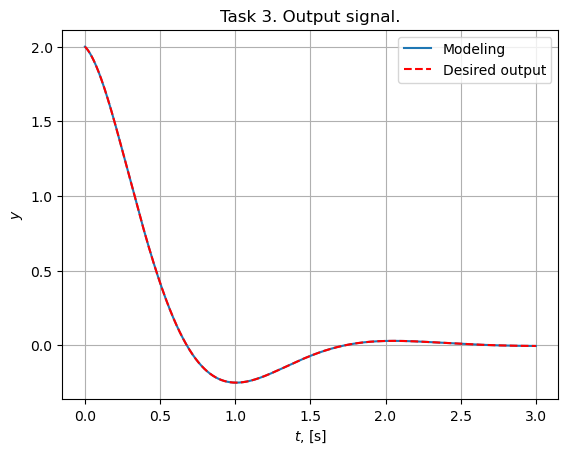
\includegraphics[width=0.7\textwidth]{../../plots/task_3_2.png}
    \caption{Ошибка сходимости}
    \label{fig:task_3_error_system}
\end{figure}

\begin{figure}[H]
    \centering
    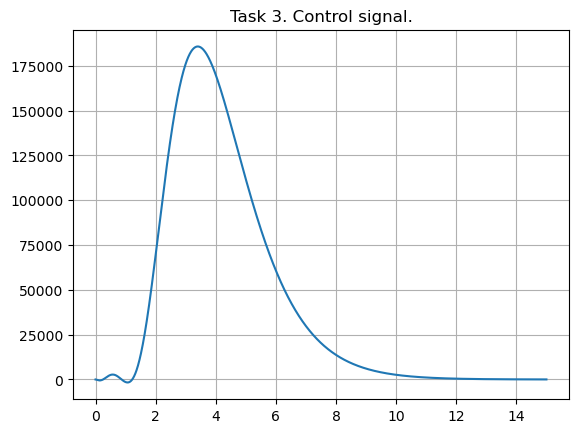
\includegraphics[width=0.7\textwidth]{../../plots/task_3_3.png}
    \caption{Управление регулятора}
    \label{fig:task_3_control_signal}
\end{figure}


\subsection{Вывод}
В рамках данного задания мы синтезировали \textbf{полное управление по выходу}, которое включает связку наблюдателя и регулятора. Мы работали с системой, которая является \textbf{полностью наблюдаемой и управляемой}, что позволило нам свободно выбирать желаемые спектры как для наблюдателя, так и для регулятора. Проведённое моделирование подтвердило успешную работу связки: наблюдатель корректно оценивал состояние системы, а регулятор обеспечивал стабилизацию системы в соответствии с заданными требованиями.
	\section{Наблюдатель пониженного порядка}

Исследуемая система описывается уравнениями:
\[
\begin{cases}
    \dot{x} = Ax + Bu, \\
    y = Cx + D,
\end{cases}
\]
где:
\begin{itemize}
    \item $x$ — вектор состояния системы,
    \item $u$ — входной сигнал (управление),
    \item $y$ — выходной сигнал.
\end{itemize}

Матрицы системы заданы следующим образом:

\[
A = \begin{bmatrix}
    5 & -7 & -5 & 1 \\
    -7 & 5 & -1 & 5 \\
    -5 & -1 & 5 & 7 \\
    1 & 5 & 7 & 5
\end{bmatrix}, \quad
B = \begin{bmatrix}
    5 \\
    7 \\
    1 \\
    9
\end{bmatrix}, \quad
C = \begin{bmatrix}
    0 & 1 & 0 & 0 \\
    1 & 0 & 0 & 0
\end{bmatrix}, \quad
D = \begin{bmatrix}
    4 \\
    2
\end{bmatrix}.
\]


\subsection{Исследование характеристик системы}

Найдём собственные числа матрицы $A$:
\[
    \sigma(A) = \{-8, 4, 8, 16\}.
\]

Проверим полные характеристики системы с помощью матриц наблюдаемости и управляемости:

\[
V = \begin{bmatrix}
    C \\
    CA \\
    CA^2 \\
    CA^3
\end{bmatrix}, \quad
    U = \begin{bmatrix}
    B & AB & A^2B & A^3B
\end{bmatrix}.
\]

Ранги матриц $V$ и $U$ равны 4:
\[
    \text{rank}(V) = 4, \quad \text{rank}(U) = 4.
\]

Матрицы являются полноранговыми, что означает, что система \textbf{полностью наблюдаема и управляема} по всем собственным числам. Из этого также следует, что система является \textbf{стабилизируемой и обнаруживаемой}.

\subsection{Синтез наблюдателя пониженного порядка}

Для наблюдателя пониженного порядка (который оценивает не все компоненты вектора состояния) выберем следующие матрицы $G$ и $Y$:

\[
G = \begin{bmatrix}
    -3 & 1 \\
    0 & -3
\end{bmatrix}, \quad
Y = \begin{bmatrix}
    1 & 0 \\
    0 & 1
\end{bmatrix}.
\]

Спектр матрицы $G$:
\[
    \sigma(G) = \{-3, -3\}.
\]

Условия для синтеза наблюдателя пониженного порядка аналогичны условиям для наблюдателя полного порядка, но используются матрицы меньшей размерности.

Решим уравнение Сильвестра для нахождения матрицы преобразования $Q$:
\[
GQ - QA = YC, \quad \rightarrow \quad Q = \begin{bmatrix}
    0.03 & -0.03 & 0.09 & -0.07 \\
    -0.02 & 0.05 & 0.07 & -0.09
\end{bmatrix}.
\]

Динамика наблюдателя описывается уравнениями:
\[
    \dot{z} = QAQ^{-1}z + QBu,
\]
\[
    \dot{\hat{z}} = G\hat{z} - Yy + (QB + YD)u.
\]

Для управления по обратной связи требуется оценка вектора состояния, которая формируется следующим образом:
\[
    u = K\hat{x}, \quad \hat{x} = \begin{bmatrix}
    C \\
    Q
\end{bmatrix}^{-1} \begin{bmatrix}
    y - Du \\
\hat{z}
\end{bmatrix}.
\]

\subsection{Синтез регулятора}

Для синтеза регулятора используем матрицы $Y$ и $G$ из предыдущего задания. Коэффициенты регулятора остаются неизменными:
\[
K = \begin{bmatrix}
    8.51 & -8.91 & -0.87 & -1.36
\end{bmatrix}.
\]


\subsection{Моделирование системы}

Проведём моделирование с начальными условиями:
\begin{itemize}
    \item Вектор состояния системы: $x(0) = \begin{bmatrix} 1 & 1 & 1 & 1 \end{bmatrix}^T$.
    \item Вектор состояния наблюдателя: $\hat{x}(0) = \begin{bmatrix} 0 & 0 & 0 & 0 \end{bmatrix}^T$.
\end{itemize}

\begin{figure}[H]
    \centering
    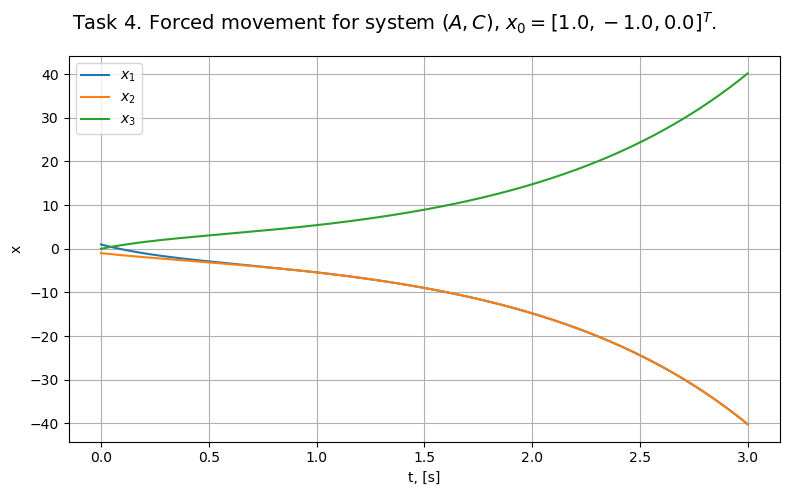
\includegraphics[width=0.7\textwidth]{../../plots/task_4_1.png}
    \caption{Состояние системы}
    \label{fig:task_4_state_system}
\end{figure}

\begin{figure}[H]
    \centering
    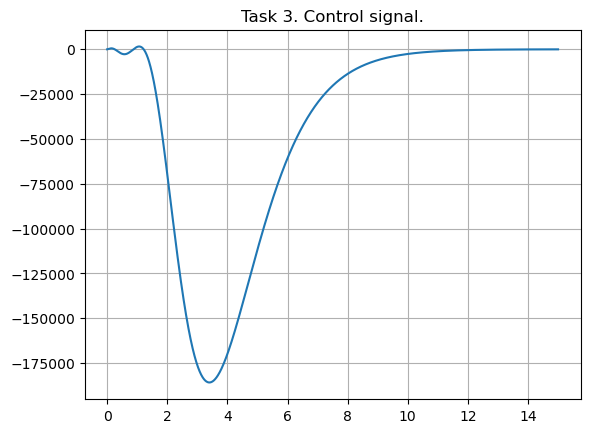
\includegraphics[width=0.7\textwidth]{../../plots/task_4_2.png}
    \caption{Управление регулятора}
    \label{fig:task_3_control_controller}
\end{figure}

\begin{figure}[H]
    \centering
    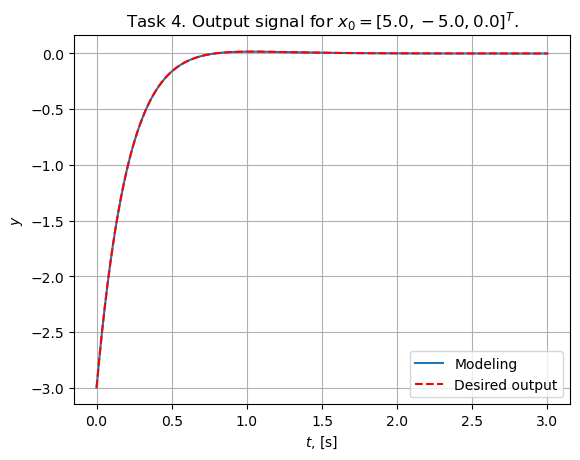
\includegraphics[width=0.7\textwidth]{../../plots/task_4_4.png}
    \caption{Ошибка наблюдателя}
    \label{fig:task_4_error_observer}
\end{figure}

Как видно из результатов моделирования, ошибка наблюдателя $e(t) = x(t) - \hat{x}(t)$ становится малой. Это означает, что наблюдатель почти сразу начинает точно оценивать состояние системы.


\subsection{Вывод}
В рамках данного задания мы синтезировали связку \textbf{модального наблюдателя пониженного порядка} и \textbf{регулятора}. Мы работали с системой, которая является \textbf{полностью наблюдаемой и управляемой}, что позволило нам свободно выбирать желаемые спектры как для наблюдателя, так и для регулятора. В отличие от полного наблюдателя, здесь мы отслеживали только \textbf{2 компоненты состояния системы} (из 4 возможных). Для этого был использован специальный подход к синтезу наблюдателя, основанный на решении \textbf{уравнения Сильвестра}, которое позволило найти матрицу преобразования $Q$.

Проведённое моделирование подтвердило успешную работу связки: наблюдатель корректно оценивал выбранные компоненты состояния системы, а регулятор обеспечивал стабилизацию системы в соответствии с заданными требованиями.


	\section{Общий вывод}
В ходе выполнения лабораторной работы был рассмотрен синтез \textbf{модального регулятора} и \textbf{наблюдателя} (полного и пониженного порядка) как по отдельности, так и в связке (стандартный линейный регулятор по выходу). Синтез осуществлялся с использованием метода \textbf{уравнения Сильвестра}. Проведённое компьютерное моделирование подтвердило корректность синтеза:
\begin{itemize}
    \item Наблюдатель успешно сходился к истинному состоянию системы.
    \item Регулятор эффективно стабилизировал систему, приводя её в положение равновесия.
\end{itemize}

\end{document}